\chapter{Fields of Application}

\section{The Elastic Stack}
\label{sec:elasticstack}
The following chapter is based on the guide of \autocite{bermand.2019}. 

The original ELK Stack by Elastic consisted of the three open source products Elasticsearch, Logstash and Kibana. As it nowadays also includes a collection of log shippers, called Beats, Elastic renamed it as the Elastic Stack.

\begin{figure}
    \centering
    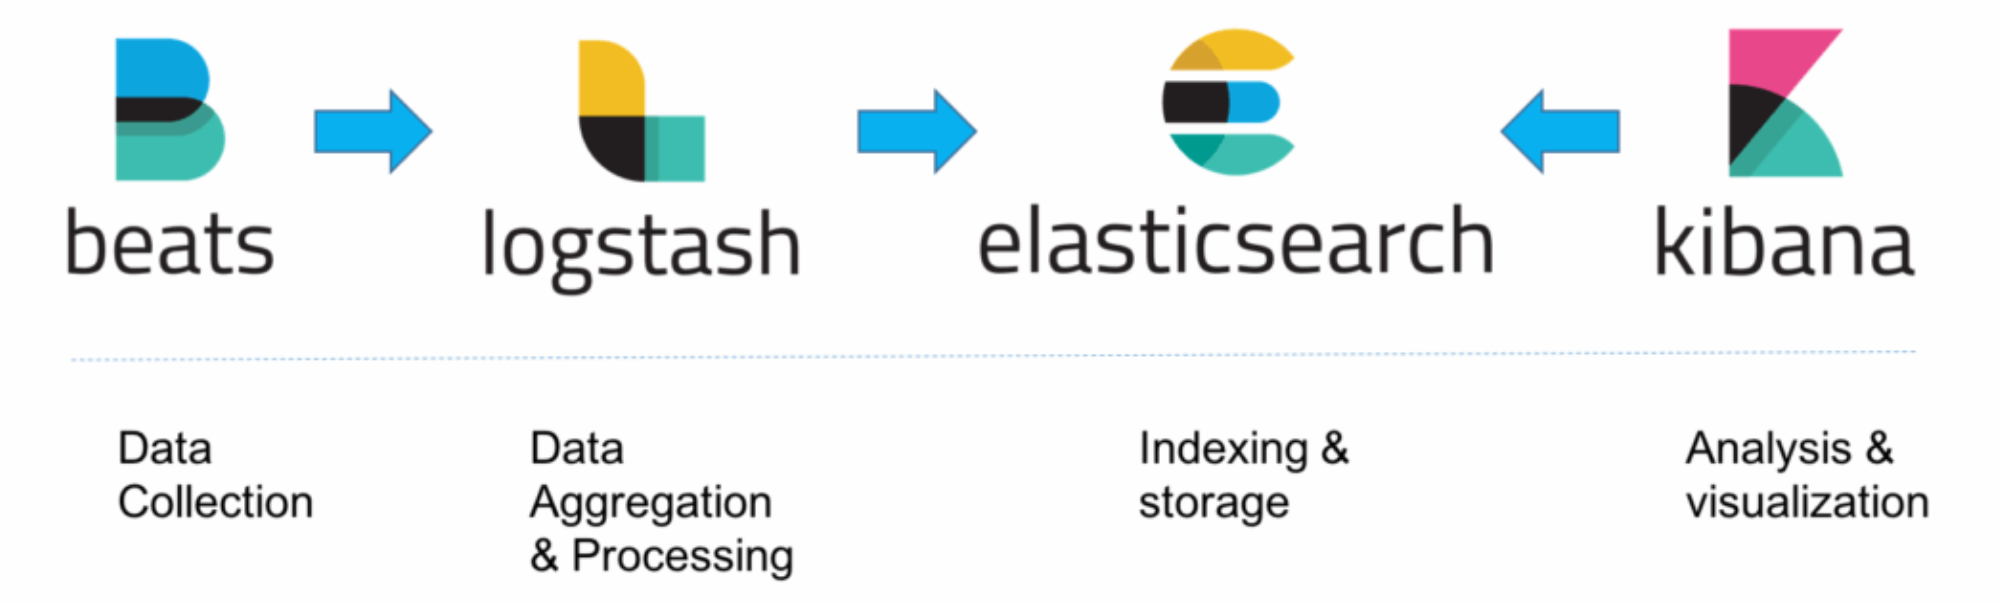
\includegraphics[width=1\textwidth]{ElasticStack.png}
    \caption{Elastic Stack overview \autocite{bermand.2019}}
    \label{fig:elasticstack}
\end{figure}
  
Figure \ref{fig:elasticstack} gives an overview on the tools included in the Elastic Stack and their tasks.

The different Beats collect logs or metrics from various sources. As these lightweight tools are written in Go, they are small as well as resource-efficient and require no dependencies.

Logstash can handle large amounts of log data provided by the Beats. The product processes the log messages and sends them to a defined storage destination in Elasticsearch.

Elasticsearch is a NoSQL document-oriented database, which provides many search capabilities and features. Its search and analytics engine is based on Apache Lucene (see chapter 3). It is responsible for indexing and storing the information received from Logstash. Elasticsearch offers an extensive RESTful API, which allows users to perform many different search queries on the data. 

Kibana provides a browser-based user interface, which allows users to easily perform search queries on the data stored in Elasticsearch. Furthermore, it enables the users to analyze their data and to visualize it using the extensive graphical capabilities of Kibana.

Overall the Elastic Stack aims to provide a reliable and scalable way to aggregate data from multiple sources, to store and to analyze it.

\section{Use Cases of the Elastic Stack}
The Elasticsearch website lists several use cases, which have been realized in different companies using one or more products from the Elastic Stack \autocite{elastic2019_02}. 

\begin{figure}
    \centering
    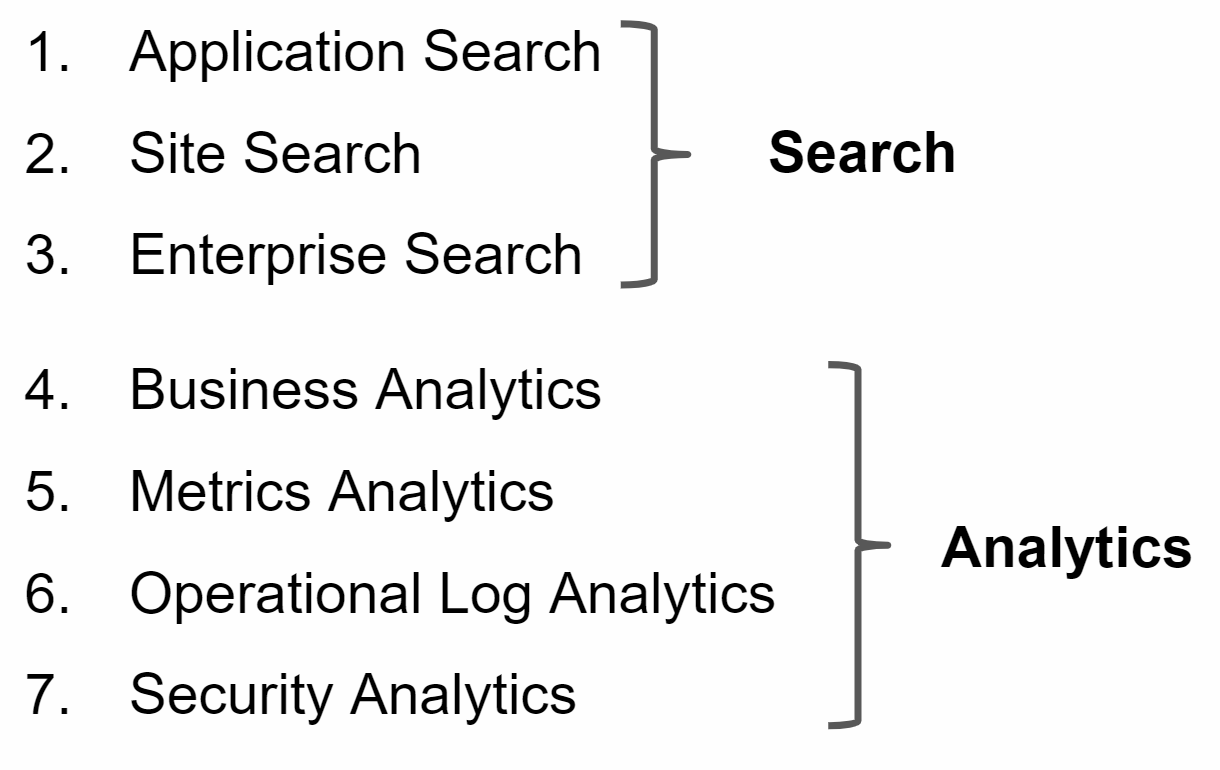
\includegraphics[width=0.5\textwidth]{UseCasesElasticStack.png}
    \caption{Overview on the different Elastic Stack use cases}
    \label{fig:estackusecases}
\end{figure}

As shown in figure \ref{fig:estackusecases}, the two main fields of application of the Elastic Stack are search and analytics, which can be divided into several subcategories. Many customers implementing the Elastic Stack, combine two or more of the subcategories \autocite{elastic2019_02}. Often, companies implement a search and an analytics use case. For example, they want to provide a nearly real-time search on their website as well as monitoring their IT systems to detect security breaches. 

In the following, an example implementation for each use case subcategory will be shortly described. Details on each use case can be found on the Elasticsearch website.

\begin{enumerate}
    
    \item \underline{Application Search} \autocite{slevat.2018} \\
    The banking company Rabobank created an application that allows customers to search through their financial transactions. By using the Elastic Stack, the company was able to drastically improve the search performance.
    
    \item \underline{Site Search} \autocite{elastic2019_03} \\
    The technology blog network Engadget uses the Elastic Stack to provide a news article search functionality for its users. 

    \item \underline{Enterprise Search} \autocite{elastic2019_04} \\
    The aeronautics manufacturer Airbus created an enterprise search system to provide authorized internal and external users access to technical aircraft documents.  

    \item \underline{Business Analytics} \autocite{elastic2019_05} \\
    The car rental company car2go uses the Elastic Stack to monitor and visualize the connectivity and condition of the vehicles, position data, reservations and payment. Furthermore, the realized system allows the company to analyze fraud cases.

    \item \underline{Metrics Analytics} \autocite{elastic2019_06} \\
    The game developer Blizzard Entertainment implemented an analytics system using the Elastic Stack to identify potential problems quickly and to reduce the reaction time if a problem occurs. By monitoring important metrics, the company gains insights into which game features are working best and which features have to be improved.

    \item \underline{Operational Log Analytics} \autocite{elastic2019_07} \\
    The healthcare IT supplier Cerner uses the Elastic Stack to index and analyze events in near real-time and to send out alerts to the responsible emergency team in case of a severe event. This allows the company to increase the stability and reliability of its IT infrastructure. 
    
    \item \underline{Security Analytics} \autocite{paquettem.2018} \\
    A group of five big US universities, led by the Indiana University, uses an Elastic Stack solution that ingests, correlates and analyzes vast quantities of information to detect security breaches and cyber threats in their IT systems. This enables the universities to protect their students, faculties and staff from cyber attacks.

\end{enumerate}
